\documentclass{article}
\usepackage[utf8]{inputenc}
\usepackage{amsmath, amssymb, amsthm}
\usepackage{pgf,tikz,pgfplots}
\usepackage{mathrsfs}
\usepackage{hyperref}

\pgfplotsset{compat=1.15}

\tikzset{every picture/.style={line width=0.75pt}} %set default line width to 0.75pt        

\newcommand{\diag}{\mathrm{diag}}
\newcommand{\Aut}{\mathrm{Aut}}
\newcommand{\Inn}{\mathrm{Inn}}
\newcommand{\Ad}{\mathrm{Ad}}
\newcommand{\ad}{\mathrm{ad}}
\newcommand{\Tor}{\mathbb{T}}
\newcommand{\Real}{\mathbb{R}}
\newcommand{\Comp}{\mathbb{C}}
\newcommand{\Quar}{\mathbb{H}}
\newcommand{\gSO}{\mathrm{SO}}
\newcommand{\gSU}{\mathrm{SU}}
\newcommand{\gO}{\mathrm{O}}
\newcommand{\gU}{\mathrm{U}}
\newcommand{\gSp}{\mathrm{Sp}}

\newtheorem{theorem}{Theorem}

\title{Highlights of elementary Lie theory\footnote{This is a quick walkthrough of some important ideas in Lie theory. For a fuller treatment (in-progress), see: \url{https://thewindingnumber.blogspot.com/p/1203.html} (for Lie theory) and \url{https://thewindingnumber.blogspot.com/p/2204.html} (for Topology).}}
\author{Abhimanyu Pallavi Sudhir}
\date{October 2019}

\begin{document}

\maketitle

\tableofcontents

\section{Lie groups and algebras; exponential map}

The motivation for the theory of Lie groups comes from a fundamental topological insight: some vague notion of ``wiggle room'' often has a lot of the properties of the notion of cardinality -- the classic example of this in topology is \emph{compact spaces}, which have a finite ``wiggle room'', generalising how finite sets have a finite cardinality. Even though the closed interval $[0,1]$ has the same cardinality as $\Real$, it is often ``visualised'' in a similar way to a set like $\{0,1\}$.

Well, the same insight should be available in group theory -- for instance, the circle group is analogous to a cyclic group, $(\Real,+)$ is analogous to $(\mathbb{Z},+)$, etc. The key notion we want to make sense of this is a \emph{real-index power} (that is at least sometimes defined) on Lie groups generalising the standard integer-index power that is available to us for free.

A definition of real powers requires some notion of a parameterisation, which exists as input to an exponential function. The interesting fact about Lie groups is that they come with a very natural source of this parameterisation: the tangent space at the identity. 

\vspace{15pt}

\begin{figure}[!h]
\centering
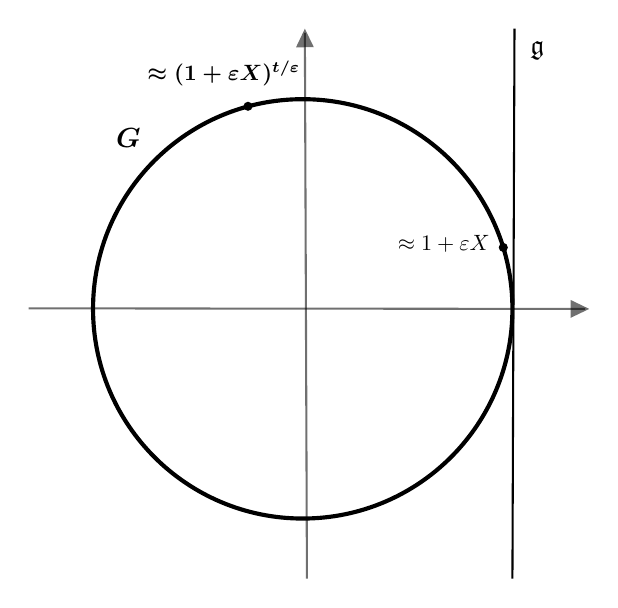
\begin{tikzpicture}[x=0.75pt,y=0.75pt,yscale=-1,xscale=1]
%\path (0,423.3999938964844); %set diagram left start at 0, and has height of 423.3999938964844

%Shape: Circle [id:dp04374042404288758] 
\draw  [fill={rgb, 255:red, 0; green, 0; blue, 0 }  ,fill opacity=1 ] (369,181.65) .. controls (369,180.74) and (369.74,180) .. (370.65,180) .. controls (371.56,180) and (372.3,180.74) .. (372.3,181.65) .. controls (372.3,182.56) and (371.56,183.3) .. (370.65,183.3) .. controls (369.74,183.3) and (369,182.56) .. (369,181.65) -- cycle ;
%Shape: Circle [id:dp7895348759813148] 
\draw  [fill={rgb, 255:red, 0; green, 0; blue, 0 }  ,fill opacity=1 ] (246,113.65) .. controls (246,112.74) and (246.74,112) .. (247.65,112) .. controls (248.56,112) and (249.3,112.74) .. (249.3,113.65) .. controls (249.3,114.56) and (248.56,115.3) .. (247.65,115.3) .. controls (246.74,115.3) and (246,114.56) .. (246,113.65) -- cycle ;
%Shape: Circle [id:dp8381206521964208] 
\draw  [line width=1.5]  (172.99,211.25) .. controls (172.99,155.45) and (218.22,110.22) .. (274.02,110.22) .. controls (329.81,110.22) and (375.05,155.45) .. (375.05,211.25) .. controls (375.05,267.04) and (329.81,312.27) .. (274.02,312.27) .. controls (218.22,312.27) and (172.99,267.04) .. (172.99,211.25) -- cycle ;
%Straight Lines [id:da8663363596886942] 
\draw    (376.05,76.27) -- (375.05,341.27) ;

%Straight Lines [id:da5806673160257454] 
\draw [color={rgb, 255:red, 0; green, 0; blue, 0 }  ,draw opacity=0.56 ]   (142,211) -- (410.05,211.27) ;
\draw [shift={(412.05,211.27)}, rotate = 180.06] [fill={rgb, 255:red, 0; green, 0; blue, 0 }  ,fill opacity=0.56 ][line width=0.75]  [draw opacity=0] (8.93,-4.29) -- (0,0) -- (8.93,4.29) -- cycle    ;

%Straight Lines [id:da8769810999963519] 
\draw [color={rgb, 255:red, 0; green, 0; blue, 0 }  ,draw opacity=0.56 ]   (276.05,341.27) -- (275.05,78.27) ;
\draw [shift={(275.05,76.27)}, rotate = 449.78] [fill={rgb, 255:red, 0; green, 0; blue, 0 }  ,fill opacity=0.56 ][line width=0.75]  [draw opacity=0] (8.93,-4.29) -- (0,0) -- (8.93,4.29) -- cycle    ;

% Text Node
\draw (190,129) node   {$\boldsymbol{G}$};
% Text Node
\draw (387,87) node   {$\mathfrak{g}$};
% Text Node
\draw (342,180) node [scale=0.8]  {$\approx 1+\varepsilon X$};
% Text Node
\draw (236,98) node [scale=0.8]  {$\boldsymbol{\approx ( 1+\varepsilon X)^{t/\varepsilon }}$};
\end{tikzpicture}
\caption{Lie algebras and the exponential map}
\label{fig:exp}
\end{figure}

Fig.~\ref{fig:exp} shows the intuition for why this makes sense -- a group element infinitesimally close to the identity, $1+\varepsilon X$ (where $X$ is some basis element in the tangent space) exponentiates by a real power $t/\varepsilon$ to the group element $(1+\varepsilon X)^{t/\varepsilon}$. With infinitesimal $\varepsilon$, this can be considered the definition of $\exp{tX}$ -- and it's easy to check that this is equivalent to the ``power series'' definition.

(It's reasonable to ask how we can perform such ``addition'' between the group identity and vector space elements. Well, right now, we're considering the group and its Lie algebra to both be embedded in some $GL(\Real^n)$ -- we can then figure out what the properties are that an ``abstract'' Lie group or algebra ought to satisfy.)

\section{Lie bracket; Lie homomorphisms}

Much of the motivation behind Lie theory has to do with translating between ideas in the group and the tangent space -- the ultimate hope is that we may be able to equip the tangent space with enough structure that it could characterise the Lie group (or at least its local behaviour) completely. Certainly for an Abelian Lie group just the linear space structure suffices, as $\mathrm{exp}$ is a local homeomorphism in this case. So it's sensible to expect that the remaining structure in the general case has something to do with the non-commutativity of the group.

There are two equivalent ways to see the Lie bracket -- the first makes the connection to non-commutativity more clear, but the second perhaps better illustrates the importance of the operation in connection to the conjugation map.
\begin{itemize}
    \item $[X,Y]$ is the second-derivative at the identity of the commutator curve $e^{tX}e^{tY}e^{-tX}e^{-tY}$. Because the first-derivative is zero, replacing $t$ with $\sqrt{t}$ shows that it is a member of the Lie Algebra.
    \item The differential of $\Ad:G\to\Aut(G):=g\mapsto \lambda h.\ ghg^{-1}$ (the ``Adjoint map'' homomorphism) is $\ad:TG\to T\Aut(G):= X \mapsto [X,\cdot]$. One immediate consequence of this understanding is that $\ad$ is a Lie Algebra homomorphism, and thus preserves the Lie bracket: $\ad([X,Y])=[\ad(X), \ad(Y)]$ (this is a form of the \emph{Jacobi identity}).
\end{itemize}

Note that we haven't yet abstractly defined a Lie algebra or a Lie algebra homomorphism. When writing down \emph{Lie's fundamental theorems}, it will be convenient to define a Lie algebra as simply a vector space equipped with a Lie bracket (and thus a homomorphism of Lie algebras preserves this Lie bracket), and the Lie bracket as a bilinear operator that is antisymmetric and satisfies the Jacobi identity -- but Lie's theorems are what serve as the \emph{motivation} for this definition.

Another example of a Lie algebra homomorphism induced by a Lie group homomorphism is the automorphism of conjugation on the Lie algebra, $\Ad(g)(X)=gXg^{-1}$, defined as the derivative of a conjugation automorphism $Ad(g)(h)=ghg^{-1}$. This map defines the ``adjoint representation'' of the Lie group, although only faithful iff the group has trivial center. If we want to understand $\Ad(g)$ as a ``rotation'' transformation, we would need to introduce the \emph{Killing form} (in fact, for simple Lie algebras, this is the \emph{unique} $\Ad$-invariant bilinear form up to scaling) -- we can then see, e.g. that $[X,Y]$ (the tangent to the orbit of $Y$ under conjugation by a curve with derivative $X$ at 0) is normal to $X$.

We can write down other examples of correspondences between Lie groups and their Lie algebras:

\begin{itemize}
    \item A \emph{subalgebra} of a Lie algebra is the tangent Lie algebra to a a Lie subgroup -- one can confirm that it is a linear subspace closed under the Lie bracket.
    \item An \emph{ideal} of a Lie algebra is the tangent Lie algebra to a normal subgroup -- one can confirm that $\mathfrak{i}$ is an ideal of $\mathfrak{g}$ iff $[\mathfrak{g},\mathfrak{i}]\subseteq\mathfrak{i}$, or equivalently iff it is the kernel of a Lie algebra homomorphism.
    \item The \emph{centre} of a Lie algebra is the tangent space to the centre of the group -- equivalently, the largest subalgebra (in fact ideal) $\mathfrak{z}$ such that $[\mathfrak{g},\mathfrak{z}]=0$.
\end{itemize}

It is then reasonable to ask if these implications go both ways -- i.e. is every Lie algebra homomorphism the differential of a Lie group homomorphism; is every Lie subalgebra the tangent to a subgroup? This questions will be the subject of Lie's fundamental theorems.

\section{Exceptional isomorphisms}

Linear algebra is really simple on the whole isomorphism question -- two linear spaces (over the same field) are isomorophic iff they have the same dimension. Things are much harder in topology and group theory.

Well, at least with the classical Lie groups, they are easy to categorise, so if we can define some invariants, we can perhaps decide what groups definitely aren't isomorphic and then worry about the remaining ones. Here are three invariants: dimension, center, rank (dimension of maximal torus).

The classical Lie groups we are interested in are the connected ones -- so not $\gO(n)$ -- we can start with $\gSO(n)$ , $\gSU(n)$, $\gU(n)$, $\gSp(n)$. The first thing we can do is look at how rank and dimension vary in each of these series: the rank of $\gU(n)$ is always $n$  while its dimension is $n^2$. In $\gSU(n)$, the subgroup of diagonal matrices loses a degree of freedom, thus its rank is always $n-1$ while its dimension is $n^2-1$. The dimension of $SO(n)$ is $n(n-1)/2$ while its rank -- well, you need two real dimensions to make a torus, so its rank is $\lfloor n / 2\rfloor$. The Symplectic group is a bit harder to visualise, but one can consider the diagonal matrices with $(1,i)$ entries to be a maximal torus so that the rank of $\gSp(n)$ is $n$ -- and of course, its dimension can easily be seen to be $n(2n+1)$.

Classifying by rank, this means for rank at least 4, 
$$\dim \gU<\dim \gSU<\dim \gSO(\mathrm{even})<\dim\gSO(\mathrm{odd})=\dim\gSp$$
Well, for odd $n$, $\gSO(n)$ has trivial center while $\gSp(n)$ has center $\{I, -I\}$. We can then look at the finite number of groups in ranks 1, 2 and 3 and confirm that the only cases where all three invariants are the same are:
\begin{itemize}
    \item $\gSO(2)$ and $\gU(1)$
    \item $\gSU(2)$ and $\gSp(1)$
\end{itemize}
In the first case, the isomorphism is simply the canonical real form of complex matrices -- in the second, the isomorphism is simply the canonical complex form of quaternion matrices. So these cases indeed are isomorphisms. So these are the only isomorphisms we can write of the stated groups.

One could introduce some new Lie groups by quotienting over normal subgroups -- well, in particular it happens that all the quotients over the centres (which are equivalently the inner automorphism groups) of the mentioned classical Lie groups: $\Inn(\gSO(n))$, $\Inn(\gSU(n))$, $\Inn(\gU(n))$, $\Inn(\gSp(n))$ are  simple.

\section{Lie's theorems: aka ``Why stop there?''}

There are two decisions in the definition of a Lie algebra you'll find online that seem rather un-motivated: (1) why is the Lie bracket the only structure you endow the tangent space with to make a Lie algebra? (2) why are bilinearity, anticommutativity and the Jacobi identity sufficient to characterise a Lie algebra?

The answers, as you may expect, are: (2) all such algebras are Lie algebras to a Lie group, (1) the group (up to connectedness, coverings) is determined by just this information. These are Lie's third and second theorems (up to a special case) respectively:

\begin{enumerate}
    \item\textbf{Lie's first theorem} -- This refers to the relatively easy facts that (a) the Lie algebra of a Lie group is a Lie algebra, and two Lie groups have the same Lie algebra iff their connected components have the same universal cover, and (b) a homomorphism of Lie groups induces a homomorphism of their Lie algebras. The next two theorems are essentially the converse of (b) and (a) respectively.
    \item\textbf{Lie's second theorem} -- For a Lie algebra homomorphism $L:TG\to TH$, if $G$ is simply-connected, there is a unique Lie group homomorphism $\ell: G\to H$ such that $L=d\ell$.
    \item\textbf{Lie's third theorem} -- Every Lie algebra is the Lie algebra of a unique simply-connected Lie group.
\end{enumerate}

Together, these form the \textbf{Lie correspondence}. They have various consequences of a similar nature, e.g. the correspondence between subgroups and subalgebras, normal subgroups and ideals, centers and centers, abelian Lie groups and abelian Lie algebras, etc.

The first theorem is elementary. The second theorem can be proven quite trivially using the Baker-Cambell-Hausdorff theorem (below). The third theorem is quite hard.

\begin{theorem}
Baker-Cambell-Hausdorff theorem (existence): The power series of $\log(e^Xe^Y)$ (which is defined on some neighbourhood of the identity) is expressible purely in terms of the nested commutators of $X$, $Y$.
\end{theorem}
\begin{proof}
We reproduce the proof by Eichler (1967) \cite{eichler}. Group the terms by degree as $F_n$ in the expansion of $\log(e^Xe^Y)$, i.e.
$$\mu(X,Y)=\sum_{n=1}^\infty F_n(X,Y)$$
Noting that $F_1(X,Y)=X+Y$ and $F_2(X,Y)=\frac12[X,Y]$, we will prove by strong induction that each $F_n$ is a Lie polynomial. Suppose that all $F_m$ are Lie polynomials for $m<n$. Then the main ``stroke of genius'' behind the proof is to nest:
$$({e^X}{e^Y}){e^Z} = {e^X}({e^Y}{e^Z})$$
$$\sum {{F_i}\left( {\sum {{F_j}(X,Y)} ,Z} \right)}  = \sum {{F_i}\left( {X,\sum {{F_j}(Y,Z)} } \right)}$$
Looking at terms of degree $n$ only, all terms except $F_n(X,Y)+F_n(X+Y,Z)$ on the left-hand-side and all terms except $F_n(X,Y+Z)+F_n(Y,Z)$ are nestings of $F_m$'s of lower degree and are thus Lie polynomials themselves. Thus the difference between the aforementioned exceptions is a Lie polynomial, which we write as:
\begin{equation}\label{0}
    F_n(X,Y)+F_n(X+Y,Z)\sim F_n(X,Y+Z)+F_n(Y,Z)
\end{equation}
And $\sim$ can be checked to be an equivalence relation. Showing from here that $F_n(X,Y)\sim 0$ is like a 15 puzzle of sorts. The first couple of manipulations are at least somewhat predictable -- considering the cases $Z=-Y$ and $X=-Y$ respectively yields:
\begin{equation}\label{1}
    F_n(X,Y)\sim-F_n(X+Y,-Y)
\end{equation}
\begin{equation}\label{2}
    F_n(X,Y)\sim-F_n(-X,X+Y)
\end{equation}
One can check that applying either condition to itself transitively just yields a trivial result. But we can apply Eq.~\eqref{1} and Eq.~\eqref{2} alternatingly to obtain:
$$F_n(X,Y)\sim-F_n(-Y,-X)$$
Since $F_n$ is a iso-degree polynomial in $X$ and $Y$ of degree $n$, this is the same as:
\begin{equation}\label{3}
    F_n(X,Y)\sim (-1)^nF(Y,X)
\end{equation}
We may also consider in Eq.~\eqref{0} the cases $Z=-\frac12 Y$ and $X=-\frac12 Y$ (how to motivate this choice -- I have no clue -- the thing it simplifies to isn't very encouraging either) and similarly apply the results alternatingly to obtain:
\begin{align*}
    {F_n}(X,Y) &\sim {F_n}(\frac{1}{2}X,\frac{1}{2}Y) - {F_n}( - \frac{1}{2}X,\frac{1}{2}X + \frac{1}{2}Y)\\ 
    &\ \ \ \ - {F_n}(\frac{1}{2}X + Y, - \frac{1}{2}Y) + {F_n}(\frac{1}{2}X + Y, - \frac{1}{2}X - \frac{1}{2}Y)
\end{align*}
Simplifying with Eq.~\eqref{1} and Eq.~\eqref{2} in third and fourth, and second, terms of the right-hand-side (once again, I cannot motivate this choice) respectively:
$$(1-2^{1-n})F_n(X,Y)\sim 2^{-n}F_n(X+Y,Y)-2^{-n}F_n(Y,X+Y)$$
Simplifying with Eq.~\eqref{3},
\begin{equation}\label{4}
    (1-2^{1-n})F_n(X,Y)\sim 2^{-n}(1+(-1)^n)F_n(X+Y,Y)
\end{equation}
Now successively apply Eq.~\eqref{2} and Eq.~\eqref{4} to $F_n(X,-Y)$ and iterate the result:
\begin{align*}
    F_n(X,-Y)&\sim -F_n(X-Y,Y)\\
      &\sim -2^{-n}(1+(-1)^n)(1-2^{1-n})^{-1}F_n(X,Y)\\
    F_n(X,Y)&\sim 2^{-2n}(1+(-1)^n)^2(1-2^{1-n})^{-2}F_n(X,Y)
\end{align*}
Confirming that this coefficient on the right-hand-side is never equal to 1 for $n>2$, this implies $F_n(X,Y)$ is Lie.
\end{proof}

\section{Examples}
\subsection{Special Orthochronous Indefinite Orthogonal Group}
Preliminary definitions and facts:
\begin{itemize}
    \item The indefinite orthogonal group $\gO(m,n)$ is the group of matrices that preserve the Minkowski form $\diag(m, n)$(diagonal matrix of $m$ $1$s, $n$ $-1$s).
    \item With $\gO(n)$, simply restricting to $\gSO(n)$ is enough to eliminate all reflections and produce a connected group, because an even number of reflections compose to a rotation. But with the indefinite orthogonal group, we may not want 180-degree rotations between time and space dimensions in our ``restricted'' Lorentz group.
    \item So while we can define $\gSO(m,n):=\{A\in \gO(m,n)\mid \det A = 1\}$, it is perhaps more useful to define 
    $$\gSO^+(m,n):=\{A\in \gO(m,n)\mid \det A = 1, \det A_t > 0\}$$
    The challenge is to prove that this is a group.
    \item There is a tedious ``algebraic'' proof of this in the case where either $m=1$ or $n=1$. But this does not generalise (see \cite{omn}).
\end{itemize}
The key idea comes from the physical insight that we're looking for precisely the transformations that an initially stationary observer can continuously boost or rotate into -- i.e. we need to prove that $\gSO^+(m,n)$ forms the identity component of $\gO(m,n)$. It is clear (from considering suitable homomorphisms) that it is a union of connected components, and one may use the cos-cosh presentation of the elements to show path-connectedness.

\subsection{Parallel parking}

Lie theory happens to be useful in control theory, where one is required to study the motion of a system with some given degrees of freedom. An elementary example of such a system is driving -- the set of possible motions of the car forms a Lie group. Fig.~\ref{fig:car} shows the degrees of freedom of a car: $(x,y)$ is the position of the steering, $\phi$ is the angle of the car from the horizontal (to determine the position of the back of the car) and $\theta$ is the steering angle -- so the configuration space of the car is $\Real^2\times\Tor^2$.

We can study the Lie algebra of the system based on the two permitted motions of the car. The first is infinitesimal steering, given by 
$$\mathrm{Steer}=\partial/\partial\theta$$ 
The second is infinitesimal driving, which moves the steering forward -- one can check that this pulls $(x,y)$ forward by $\varepsilon(\sin(\theta+\phi),-\cos(\theta+\phi))$ and increases $\phi$ by $\varepsilon(-\cos\theta)$, so:
$$\mathrm{Drive}=\sin(\theta+\phi)\frac{\partial}{\partial x}-\cos(\theta+\phi)\frac{\partial}{\partial y}-\cos(\theta)\frac{\partial}{\partial\phi}$$
What's really interesting is this:
$$[[\mathrm{Steer},\mathrm{Drive}],\mathrm{Drive}] = \sin\phi\frac{\partial}{\partial x}-\cos\phi\frac{\partial}{\partial y}$$
Which is precisely the derivation corresponding to a \emph{parallel-slide}. What this means is that the following sequence of tiny motions, each with order $\varepsilon$:
$$\text{Steer, Drive, }\overline{\text{Steer} }\text{, }\overline{\text{Drive}}\text{, Drive, }\overline{\text{Steer}}\text{, }\overline{\text{Drive}}\text{, Steer, Drive, }\overline{\text{Drive}}$$
(Where an overline represents reverse-direction) Or equivalently:
$$\text{Steer, Drive, }\overline{\text{Steer}}\text{, }\overline{\text{Steer}}\text{, }\overline{\text{Drive}}\text{, Steer}$$
Produces a parallel-slide of order $\varepsilon^3$. You can confirm with a pencil or something that this is correct.

\begin{figure}
\centering
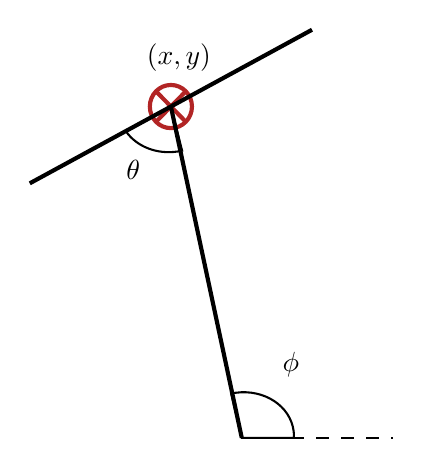
\begin{tikzpicture}[x=0.75pt,y=0.75pt,yscale=-1,xscale=1]
%uncomment if require: \path (0,300); %set diagram left start at 0, and has height of 300
%Flowchart: Summing Junction [id:dp7518038923628898] 
\draw  [color={rgb, 255:red, 178; green, 37; blue, 37 }  ,draw opacity=1 ][line width=1.5]  (283,84.6) .. controls (283,78.86) and (287.54,74.2) .. (293.15,74.2) .. controls (298.76,74.2) and (303.3,78.86) .. (303.3,84.6) .. controls (303.3,90.34) and (298.76,95) .. (293.15,95) .. controls (287.54,95) and (283,90.34) .. (283,84.6) -- cycle ; \draw  [color={rgb, 255:red, 178; green, 37; blue, 37 }  ,draw opacity=1 ][line width=1.5]  (285.97,77.25) -- (300.33,91.95) ; \draw  [color={rgb, 255:red, 178; green, 37; blue, 37 }  ,draw opacity=1 ][line width=1.5]  (300.33,77.25) -- (285.97,91.95) ;
%Straight Lines [id:da2299910067649651] 
\draw [line width=1.5]    (293.15,84.6) -- (327.3,244.2) ;


%Straight Lines [id:da47035986320225187] 
\draw [line width=1.5]    (225.15,121.6) -- (361.15,47.6) ;


%Straight Lines [id:da7731294417249341] 
\draw  [dash pattern={on 4.5pt off 4.5pt}]  (327.3,244.2) -- (400.3,244.2) ;


%Shape: Pie [id:dp11689632348659607] 
\draw   (322.2,222.87) .. controls (322.91,222.72) and (323.64,222.6) .. (324.37,222.5) .. controls (338.16,220.64) and (350.66,228.84) .. (352.27,240.83) .. controls (352.43,241.96) and (352.48,243.09) .. (352.43,244.2) -- (327.3,244.2) -- cycle ;
%Shape: Pie [id:dp9209684174157633] 
\draw   (298.55,105.85) .. controls (297.85,106.01) and (297.13,106.15) .. (296.39,106.26) .. controls (286.16,107.79) and (276.57,103.75) .. (271.58,96.66) -- (293.15,84.6) -- cycle ;

% Text Node
\draw (351,209) node   {$\phi $};
% Text Node
\draw (275,115) node   {$\theta $};
% Text Node
\draw (297,61) node   {$( x,y)$};
\end{tikzpicture}
\caption{Degrees of freedom of a car}
\label{fig:car}
\end{figure}

\section{Summary}

Here is a summary of some important insights into various Lie-theoretic ideas:

\begin{itemize}
 \item The notion of a \textbf{Lie group} itself -- the idea comes from wanting to generalise what we know about discrete groups to more complicated contexts where the ``manifold'' structure of the group allows us to do so. Examples: \textbf{compactness} generalises finiteness, \textbf{one-parameter groups} generalise cyclic groups, etc.
 \item The \textbf{exponential map} -- For one-parameter groups to generalise cyclic groups, we need a ``generalisation'' of the group power to allow ``real-index powers''. The general way to define a \textbf{real power} is through the exponential map. Well, this real power stuff isn't \emph{always} defined as it turns out (you need the exponential map to be surjective), but our motivation does explain why it "makes sense" that the \textbf{exponential map is surjective in the connected abelian case} (because then, the Lie algebra is basically a co-ordinate system on the Lie group -- I'm aware exponential co-ordinates are defined in more generality, but it's certainly more well-behaved here).
 \item The \textbf{Lie algebra}, i.e. ``why is the logarithm/parameter space the tangent space?'' We'd like to generalise the  notion of a generator to a Lie group -- consider e.g. the circle group on the complex plane. An element near the identity generates a cyclic group, and as the element goes nearer to the identity -- as it becomes an \textbf{infinitesimal generator}, the cyclic group it approaches the entire group. Well, an element close to the identity is of the form $1+\varepsilon t X$, and generates a group element as $(1+\varepsilon tX)^{1/\varepsilon}=e^{tX}$. This is also intuition for the compound-interest limit, and for Euler's identity.
 \item The \textbf{Lie bracket} is the second-derivative of the commutator curve $\gamma(t)=e^{tX}e^{tY}e^{-tX}e^{-tY}$. Well, it's also the derivative of $\gamma(\sqrt{t})$, which proves \textbf{closure under the Lie bracket}. 
 \item The real justification for the Lie bracket, however, comes from the fundamental fact that $\mathrm{ad}:\mathfrak{g}\to\mathrm{Der}(\mathfrak{g}):=X\to[X,\cdot]$ is the differential of the adjoint map $\mathrm{Ad}:G\to\mathrm{Aut}(G):=g\mapsto\lambda x, gxg^{-1}$, which is a group homomorphism. In particular, the preservation of the Lie Bracket by the differential of a group homomorphism is precisely the \textbf{Jacobi identity}: $\mathrm{ad}([x,y])=[\mathrm{ad}(x),\mathrm{ad}(y)]$. The basic point is that we are trying to reduce Lie group problems to Lie algebra ones as much as possible, and conjugation is an important idea that we'd like to see the map induced by on the Lie algebra -- we are seeing the result of the obvious fact that $T\mathrm{Aut}(G)\subseteq\mathrm{Der}(TG)$ (and also $T\mathrm{Aut}(M)=\mathrm{Der}(M)$ -- the fact that the automorphisms of an object form a group is equivalent to the derivations on an object forming a Lie algebra). Some more examples of the ``study the Lie algebra approach'': 
     \begin{itemize}
      \item The uniqueness of the determinant as a map from $G\to \mathbb{R}-\{0\}$.
      \item An \textbf{ideal} is a subalgebra ``induced'' on the Lie algebra by a normal subgroup of the Lie group. This immediately provides the interpretation as ``kernels of Lie algebra homomorphisms'' as well as the condition $[\mathfrak{g},\mathfrak{i}]\subseteq\mathfrak{i}$. 
     \end{itemize}
 \item The idea behind the manifold-structure of a Lie group is that the flows are produced by left-multiplication by group elements, so those must be homeomorphisms. This motivation can be confirmed through various topological consequences, e.g.
 \begin{itemize}
  \item \textbf{A neighbourhood of the identity generates the connected component.} The idea behind the proof is this: if an entire open neighbourhood of the identity is contained in the subgroup, it means you can "flow in any direction" from the subgroup -- but to bring these flows to an arbitrary point of the manifold, you need left-multiplication to be a homeomorphism. 
  \item \textbf{The identity component is a (normal) subgroup.} Because left-multiplication and inversion are continuous, they cannot tear the connected component apart (generalised ``intermediate value theorem''), so it is closed under multiplication.
  \item \textbf{Compact Lie groups} -- How can a Lie group possibly ``close in on itself''? Surely we keep ``extending'' an open neighbourhood $W$ of the identity by observing that $xW$ must be in the subgroup? The idea is that these translations of $W$ form an \textbf{open cover of the group, if it has a finite subcover}, then it makes sense for the group to close in on itself. By playing around with different open neighbourhoods $W$ and taking some suitable unions, one can see that this is equivalent to the condition that every open cover has a finite subcover, i.e. the group is compact.
 \item \textbf{Characterisation of Abelian Lie groups} -- ``Compact Connected Abelian Lie Group is a torus'' is a generalisation of ``finite Abelian group is a product of cyclic groups'' -- the idea is that the exponential map "wraps" the Lie algebra around into the Lie group -- this just gives the quotient of the Lie algebra by the kernel of the exponential map, which is topologically $\mathbb{R}^n/\mathbb{Z}^n$. The characterisation of a connected Abelian Lie group as a cylinder $\mathbb{R}^{n+k}/\mathbb{Z}^k$ follows similarly.
 \end{itemize}
 \item \textbf{Lie's fundamental theorems}, consequences of the \textbf{BCH theorem}, convey the notion that nestings of the Lie bracket alone are sufficient to determine the local structure of a Lie group (I do not have an intuitive explanation of \emph{why} this is true -- of why the BCH theorem makes sense). The ``up to \textbf{simply connectedness}'' condition can be readily understood -- it's obvious why the Lie algebra cannot see disconnectedness; the reason it cannot see covering spaces is that the is the quotient of its universal cover by a discrete subgroup, and an application of the fundamental theorem of homomorphisms and the fact that the Lie algebra of a discrete subgroup is trivial implies our result.
 \item The \textbf{Killing form} is the natural way to define an $\Ad$-invariant bilinear form on a Lie algebra, in fact it is unique for \textbf{simple Lie algebras}. It allows the interpretation of $\Ad$ as a ``rotation'' of the Lie algebra, as the tangents to its contours are perpendicular to the radial vectors.
\end{itemize}
Stuff not covered in this text: abstract Lie theory (representations, Ado's theorem, universal enveloping algebras); infinite-dimensional Lie theory; Killing stuff (classification of Lie groups, Cartan's criterion); abstract algebraic things (solvability, nilpotence, Levi decomposition);  differential geometry on a Lie group.

\begin{thebibliography}{19}
\bibitem{eichler}
M. Eichler, \emph{A new proof of the Baker-Cambell-Hausdorff formula}. J. Math. Soc. Japan: 40 (1-2), 1968.
\bibitem{omn}
Physics Stack Exchange (Accessed 27-09-2019): \emph{Orthochronous indefinite orthogonal group $\gO^+(m,n)$ forms a group}. \url{https://physics.stackexchange.com/q/494260}

\end{thebibliography}
\end{document}
